\documentclass[../Research.tex]{subfiles}
\usepackage[a4paper, margin=2.5cm]{geometry}
\usepackage{polski, graphicx, float, hyperref}
\setcounter{secnumdepth}{0}

\begin{document}
ArduPilot zapewnia kompleksowy zestaw odpowiednich narzędzi dla prawie każdego pojazdu i aplikacji. ArduPilot umożliwia tworzenie i korzystanie z zaufanego, autonomicznego, systemy bezzałogowych pojazdów.
Oprogramowanie działa na wielu różnych sprzętach do sterowania bezzałogowymi pojazdami wszystkich typów. W połączeniu z oprogramowaniem do kontroli naziemnej, bezzałogowe pojazdy z ArduPilot mogą mieć zaawansowane funkcje, w tym komunikację w czasie rzeczywistym z operatorem.
\subsection{Ogólna zasada działania komunikacji}
\subsubsection{Schemat blokowy}
\begin{figure}[H]
    \centering
    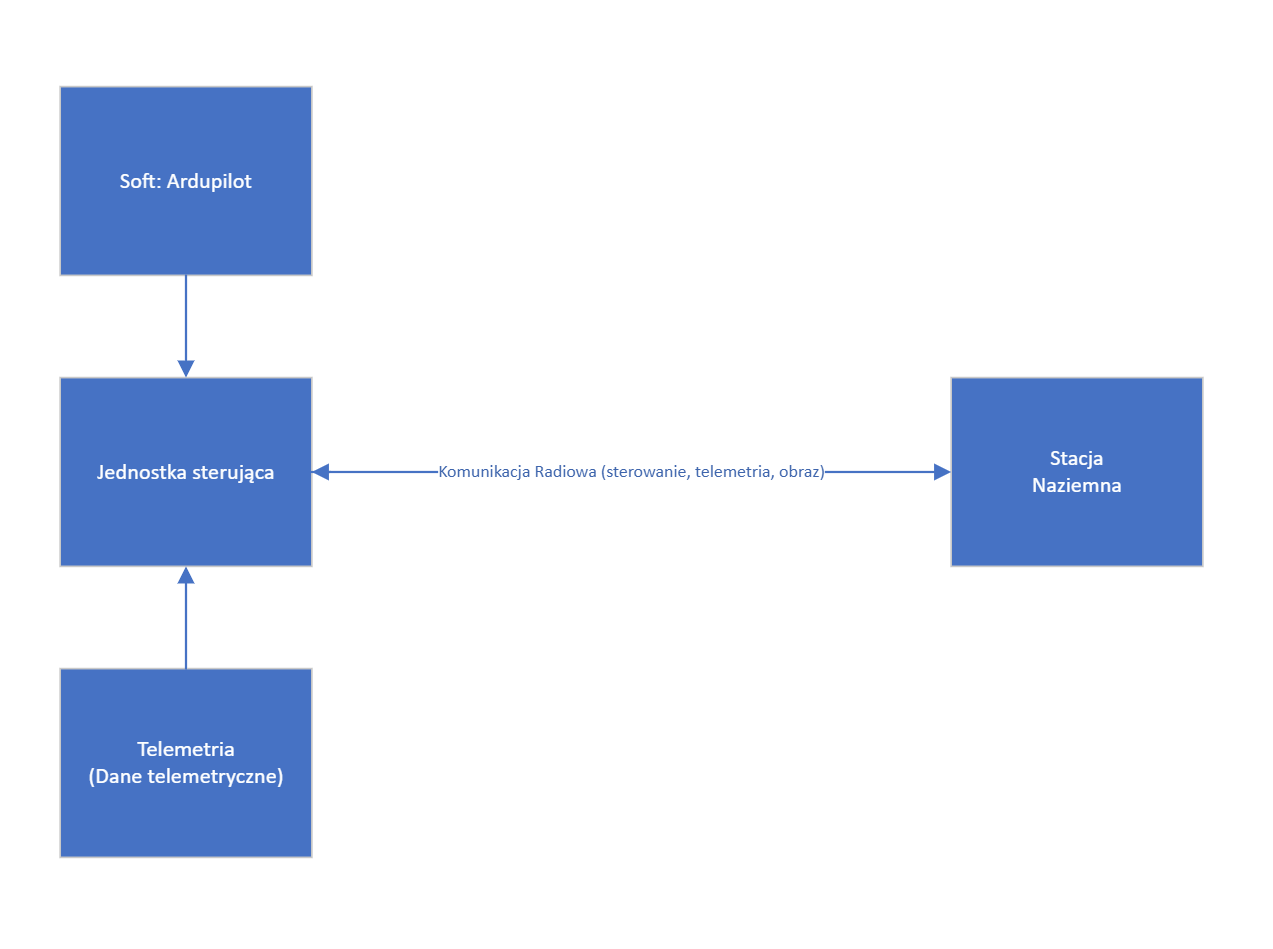
\includegraphics[width=0.7 \textwidth]{ogolna.png}
    \label{fig:obraz1}
\end{figure}

\subsection{Zmodyfikowana komunikacja po 5G}
\subsubsection{Schemat blokowy}
\begin{figure}[H]
    \centering
    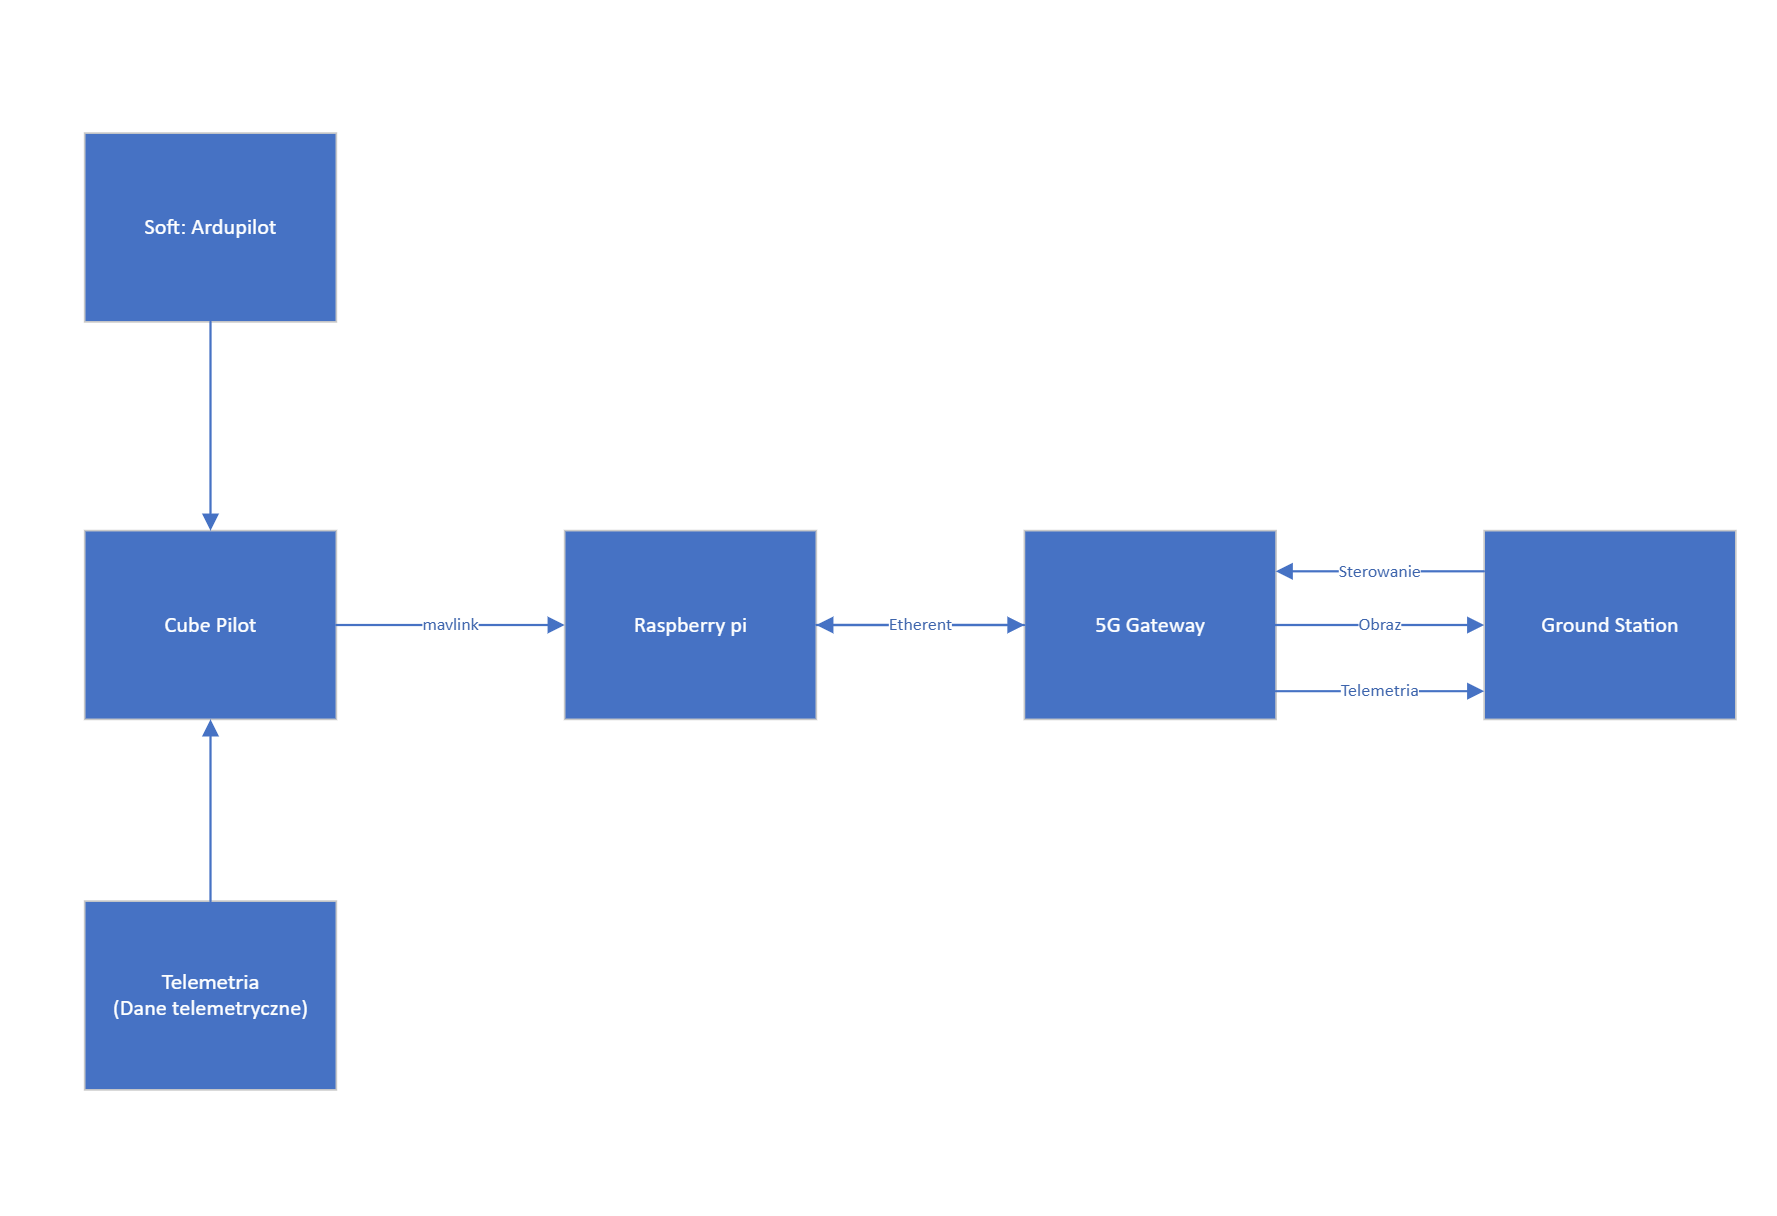
\includegraphics[width=0.7 \textwidth]{po.png}
    \label{fig:obraz2}
\end{figure}

\pagebreak

\subsection{Potokoły używane do komunikacji Ardupilota z Ground Station}
MAVLink jest protokołem szeregowym najczęściej używanym do wysyłania danych i poleceń między pojazdami a stacjami naziemnymi.
Wiadomości MAVLink można wysyłać przez prawie każde połączenie szeregowe i nie zależy to od podstawowej technologii.

\begin{enumerate}
    \item SITL/MAVProxy
    \item UDP
\end{enumerate}


Wynika z tego, że do integracji z 5G trzeba użyć protokołu UDP.


% https://ardupilot.org/dev/docs/using-sitl-for-ardupilot-testing.html#connecting-other-additional-ground-stations

\subsection{Źródła}
Strona projektu: \url{https://ardupilot.org/dev/index.html}\\
Dokumentacja: \url{https://ardupilot.org/dev/docs/using-sitl-for-ardupilot-testing.html#connecting-other-additional-ground-stations}\\
Repozytorium GitHub: \url{https://github.com/ArduPilot}\\
\end{document}
